\documentclass[resume]{subfiles}

\begin{document}
\section{Codage de source}
Aucune connaissance de la source, son rôle est de minimiser la redondance
\paragraph{Dilemme} : Si on supprime des bits dans la source, on doit en rajouter dans le canal pour augmenter la robustesse.
\subsection{Entropie}
Symboles $\lbrace a_0, a_1, a_2, \cdots, a_{n-1}\rbrace$\\
Probabilités : $\lbrace P(a_0), P(a_1), P(a_2), \cdots, P(a_{n-1})\rbrace$
Information contenue dans un message :
$$I(a_k)=-\log_2(P(a_k))\qquad [\text{bits}]$$
Entropie de la source (moyenne du contenu d'information):
$$H=\sum_{i=0}^{n-1}P(a_i)I(a_i)$$
De la source $\to$ ne pas prendre en compte si on envoie $x$ symboles. On parle uniquement de la source
\subsubsection{Combinaison de sources}
Si une source $S_3$ fait un choix entre $\textcolor{RoyalBlue}{S_1}$ et $\textcolor{OrangeRed}{S_2}$ (avec $\alpha$ la chance de $\textcolor{RoyalBlue}{S_1}$). L'entropie sera
$$\textcolor{ForestGreen}{H_3}=\alpha\Big(\textcolor{RoyalBlue}{H_1}-\log_2\left(\alpha\right)\Big)+(1-\alpha)\Big(\textcolor{OrangeRed}{H_2}-\log_2\left(1-\alpha\right)\Big)$$
Pour construire l'arbre, on multiplie les probabilités des symboles de $S_1$ par $\alpha$ et les probabilités des symboles de $S_2$ par $(1-\alpha)$
\subsection{Méthodes de codage}
\begin{enumerate}
\item Longueur fixe (comptage binaire "standard")
\item Optimal (100\% efficace) pour puissances de 2 ($\frac{1}{2}$, $\frac{1}{4}$, ..., $2\times \frac{1}{2^{n-1}}$)
\begin{center}
\begin{tabular}{ccrr}
Symbole & prob & Code A & Code B\\\hline
$s_0$ & $1/2$ & 1 & 0\\
$s_1$ & $1/4$ & 01 & 10\\
$s_2$ & $1/8$ & 001 & 110\\
$\vdots$ & $\vdots$& $\vdots$&$\vdots$ \\
$s_{n-2}$ & $1/2^{n-1}$ & 00...01 & 11...10\\
$s_{n-1}$ & $1/2^{n-1}$ & 00...00 & 11...11\\
\end{tabular}
\end{center}
Les deux codes (A et B) sont valides
\end{enumerate}
\subsection{Efficacité du code}
Entropie divisée par la longueur moyenne (déterminée à partir de la méthode de codage)
$$\frac{H}{\overline{l}}$$
Si $n$ symboles sont combinés, on divise par $n$ la longueur moyenne (pour connaître la longueur moyenne correspondant à un symbole).
\subsection{Décodage}
\paragraph{Décodage instantané} : Aucun mot-code n'est prefix d'un autre
\paragraph{Inégalité de Kraft-McMillan}
$$\sum_{i=0}^{n-1}2^{-\text{longueur}(s_i)}\neq 1\longrightarrow \text{Pas instantané}$$
Si $=1$ cela ne veut pas forcément dire que le code est instantané
\subsection{Huffman}
Attention au \textcolor{OrangeRed}{1} en \textbf{haut} ou en \textbf{bas} (les exemples sont données avec le \textcolor{OrangeRed}{1} en haut) (les deux sont utilisés dans le cours). Ensuite on construit l'arbre avec le nouvel élément "en haut" ou "en bas" (précisé dans l'exo en principe).\\
\subsubsection{Longueur moyenne}
$$\overline{l}=\sum P(a_k)\cdot \text{longueur du code}(a_k)$$
\subsubsection{Variance de la longueur}
$$\text{var}=\sigma^2=\sum P(a_k)\cdot \left(\text{longueur du code}(a_k)-\overline{l}\right)^2$$
Si on doit départager deux codes, une variance plus faible est meilleure
\subsubsection{Huffman avec nouvel élément en haut}
\begin{center}
\begin{tabular}{ccccc}
a & b & c & d & e\\
0.1 & 0.2 & 0.2 & 0.4 & 0.1
\end{tabular}
\end{center}
\begin{center}
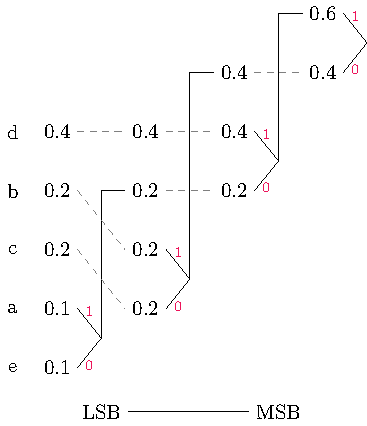
\includegraphics[scale=0.75,page=1]{drwg_4.pdf}
\\
\begin{tabular}{ccccc}
a & b & c & d & e\\
101 & 01 & 00 & 11 & 100
\end{tabular}
\end{center}

\subsubsection{Huffman avec nouvel élément en bas}
\begin{center}
\includegraphics[scale=0.75,page=2]{drwg_4.pdf}\\
\begin{tabular}{ccccc}
a & b & c & d & e\\
1101 & 10 & 111 & 0 & 1100
\end{tabular}
\end{center}



\subsection{Lempel Ziv}
\begin{figure}[H]
\centering
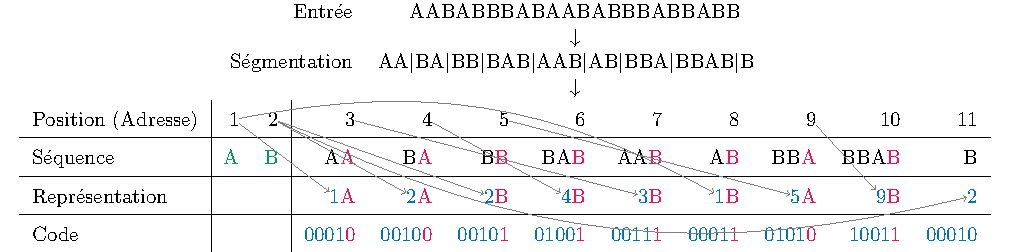
\includegraphics[width=\columnwidth]{drwg_0.pdf}
\end{figure}
\paragraph{Taux de compression} :
$$\frac{L_\text{initiale}-L_\text{finale}}{L_\text{initiale}}\ [\si{\percent}]$$
\end{document}